\documentclass[10pt]{article}
\usepackage[a4paper,textwidth=122mm,textheight=193mm,centering]{geometry}
\usepackage[T1]{fontenc}\usepackage{graphicx,booktabs,array,amssymb,amsmath,tabularx,makecell}
\usepackage[font=small,labelfont=bf,labelsep=period]{caption}\renewcommand{\figurename}{Fig.}
\graphicspath{{../figures/}}
\renewenvironment{abstract}{\small\quotation\noindent\textbf{Abstract.} }{\endquotation}
\begin{document}
\begin{center}{\large\bfseries Trust-Weighted Multi-Oracle Validation for Conflicting Land Records: A Simulation Study}\\[2mm] Author\\[6mm]\end{center}
\begin{abstract}
Blockchain land registries make records tamper-evident but cannot check whether the evidence they receive is correct. When the offices that hold land evidence disagree, a wrong ledger entry is preserved as faithfully as a correct one.

We study a synthetic pre-commit validation policy that decides whether to record a requested ownership change or to escalate it to a person. Each request bundles three simulated checks, inspired by selected conditions of Gujarat's 2026 mutation fast track: record holder, deed registration and pending proceedings. Three offices report on every check. Each report is weighted by the office's assumed authority for that check and by a trust score learned from verified outcomes. The policy does not decide title.

In simulation (six scenarios, 1,000 requests per run, 100 paired seeds, ideal feedback unless stated), the hybrid rule lowered the false-commit rate from 3.05\% to 1.09\% against majority voting in normal operation. An exploratory ablation shows the gain persists under a common coverage gate. After the most authoritative office degraded (requests 251–1000), the hybrid made fewer false commits than authority-only weighting: 5.52\% vs 6.81\%. It did the same when authority was misassigned for one check: 1.50\% vs 2.09\%.

Trust-only weighting had the lowest false-commit rate in most scenarios but committed fewer valid requests. A separate veto on reported proceedings never changed a decision under the configurations tested. In an exploratory robustness study, 67 of 68 checks of the main conclusions held across accuracy levels, shared errors between offices and noisy audits, and none reversed. Shared errors, however, raised every method's false-commit rate sharply. The data are synthetic.

\par\noindent\textbf{Keywords:}  blockchain oracles $\cdot$ land records $\cdot$ trust and reputation $\cdot$ weighted aggregation $\cdot$ e-governance $\cdot$ simulation
\end{abstract}
\section*{1 Introduction}
This paper asks how a ledger should decide, before writing, whether conflicting evidence from several offices is good enough to record a requested ownership change. It does not ask when a land transfer is legally valid. In India, entries in revenue records serve fiscal purposes and do not by themselves confer title [16]. Thakur et al. note that departments hold inconsistent data about the same land; their blockchain design defers reconciling those data to work done before deployment [1].

Gujarat's 2026 ordinance shows how one administration combines evidence for one kind of record [12]. A mutation arising from a registered sale deed may be certified the same day, without the usual notice, when three conditions hold:

\begin{itemize}
\item no change has been recorded in the record of rights for a year or more before the deed was executed;
\item everyone named in that record has executed the deed;
\item no dispute, proceeding or litigation about the land is pending before a competent authority, court or tribunal on that date.
\end{itemize}
Otherwise the normal notice route applies.

Our model borrows the shape of this rule, not its content. It simulates three checks loosely inspired by the second and third conditions, plus deed registration. It omits the record-stability condition and says nothing about title.

Blockchains, including permissioned platforms such as Hyperledger Fabric [2], have been proposed as tamper-evident land registries [1], [5]–[7], [15]. Data from outside a chain enters through oracles, which bring back trust in third parties and single points of failure [3], [8]. Oracle networks combine reporters by voting or reputation [4], [8], [10], and truth-discovery methods estimate source reliability from conflicting reports [13], [14].

Land evidence adds two complications. Each office is the natural source for a different kind of fact. And some evidence, such as a pending proceeding, plausibly calls for human review rather than a vote.

We ask five research questions:

\begin{itemize}
\item RQ1. In a synthetic setting, does combining claim-specific authority with learned reliability reduce false commits compared with majority, authority-only and trust-only weighting?
\item RQ2. How does it behave when the most authoritative office degrades, or when authority is misassigned?
\item RQ3. How do missing responses and a coverage requirement trade false commits for escalations?
\item RQ4. Does a separate veto on reported proceedings change decisions that the weighted rule would make?
\item RQ5. How do delayed and incomplete verified labels affect learned trust?
\end{itemize}
The paper makes three contributions:

\begin{enumerate}
\item A pre-commit validation policy for a three-check request bundle. It combines claim-specific authority, per-check learned trust, a coverage requirement and an optional veto, and it escalates rather than rejects.
\item A component-level comparison of five mechanisms on identical simulated worlds with hidden ground truth. Hypotheses, statistics and seeds were fixed in a protocol frozen before the final runs. Two exploratory addenda, a coverage ablation and a robustness study, were written down before they ran.
\item Evidence, under stated assumptions, on when each component helps and where the approach is fragile.
\end{enumerate}
Section 2 reviews related work and Section 3 defines the model. Section 4 describes the experiments, Section 5 the results and Section 6 their limits. Section 7 concludes.

\section*{2 Related Work}
In the sources read so far, land-registry designs rely on authorised offices to enter correct data. Oracle designs weight sources by agreement or reputation. None weights institutional sources by claim-specific authority before commitment. Table 1 summarises the comparison.

Blockchain land registries. Thakur et al. [1] describe India's land-record process and sketch a design whose nodes include revenue, registration, survey and court participants. Consensus validates transactions, not the accuracy of the underlying records, and consolidating inconsistent departmental data is deferred to pre-implementation work [1, Secs. 3.4, 6, 7.1].

Soner et al. [5] add multi-level authentication and smart-contract checks for banks and the registry. Shuaib et al. [6] place smart contracts at several registry stages. Sahai and Pandey [7] specify registry smart contracts. Khanna et al. [15] present a Hyperledger Fabric prototype that models six administrative roles and records mutations, encumbrances and disputes as chaincode states with role-aware endorsement. [VERIFY: full texts of [5]–[7]; [15] at abstract level.]

Oracles. Caldarelli [3] argues that the oracle problem matters less the more the surrounding system is trusted. For contracting and law, the review notes that a hierarchy of oracles may be needed so that illegal agreements can be reverted, without defining one [3, Sec. 5]. Al-Breiki et al. [4] compare trust features of oracle platforms, and Hassan et al. [8] review voting- and reputation-based mechanisms. Lo et al. [9] analyse oracle reliability, and Chainlink combines reports from many nodes [10].

Truth discovery and reputation. Truth-discovery methods resolve conflicting claims by jointly estimating the truth and each source's reliability [13]. DecenTruth applies the idea inside a decentralised oracle network [14]. Josang et al. [11] survey reputation systems that score parties from past behaviour. Our per-check trust is a simple reputation score of this kind, updated only from verified outcomes and combined with a fixed, claim-specific authority prior.

% Auto-generated by paper_assets/build_assets.py from saved results -- do not edit numbers by hand.
% Preamble needs: \usepackage{booktabs,array,tabularx,makecell}
\begin{table}[tb]
\centering
\caption{Comparison with related work}\label{tab:related}
\footnotesize
\setlength{\tabcolsep}{2pt}
\renewcommand{\arraystretch}{1.1}
\begin{tabularx}{\textwidth}{@{}>{\raggedright\arraybackslash}p{2.0cm}*{7}{>{\raggedright\arraybackslash}X}@{}}
\toprule
Work & Land records & Multi-source & Per-claim authority & Learned trust & Pre-commit conflict check & Escalates & Ground truth \\
\midrule
Thakur et al. [1] & yes & yes (nodes) & no & no & no (deferred) & manual & no \\
Soner et al. [5]$^\dagger$ & yes & yes & ? & ? & ? & ? & ? \\
Shuaib et al. [6]$^\dagger$ & yes & ? & ? & ? & ? & ? & ? \\
Sahai, Pandey [7]$^\dagger$ & yes & ? & ? & ? & ? & ? & ? \\
Khanna et al. [15]$^\ddagger$ & yes & yes (6 roles) & role-based & n.s. & n.s. & n.s. & n.s. \\
Chainlink [10] & no & yes (nodes) & no & reput. & aggreg. & no & no \\
Truth discovery [13] & no & yes & no & yes (unsup.) & yes & no & --- \\
DecenTruth [14]$^\ddagger$ & no & yes & no & yes (unsup.) & yes & n.s. & sim. \\
This work & synthetic & yes (3) & yes & yes (labels) & yes & yes & yes \\
\bottomrule
\end{tabularx}
\par\smallskip
\parbox{\textwidth}{\scriptsize $^\dagger$ Full text not yet read; ? = not determined. $^\ddagger$ Compared at abstract level only. n.s. = not stated in the abstract; unsup. = estimated without labels; reput. = reputation; aggreg. = aggregation of node reports; sim. = simulation; --- = not applicable to a survey.}
\end{table}

Gap. Among these sources, we found no pre-commit rule that combines claim-specific institutional authority with learned per-check reliability, escalates rather than rejects, and is evaluated against hidden ground truth. This claim is bounded to the sources listed and stays provisional until the open full-text checks are done.

\section*{3 Model}
The validator records a requested ownership change only when all three simulated checks pass on their own evidence. Otherwise it escalates to a person; it never rejects and never decides title (Fig. 1).

\begin{figure}[tb]\centering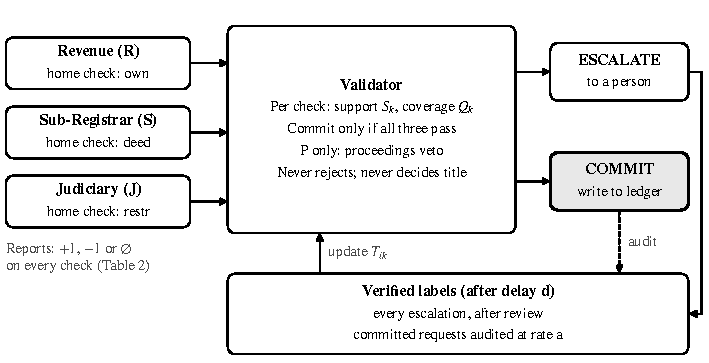
\includegraphics[width=\textwidth]{fig1_system.pdf}\caption{Validation loop. Three offices report on three checks, the validator commits a request only when all three checks pass and otherwise escalates it, and verified labels update trust.}\end{figure}
\subsection*{3.1 Scope}
A request x carries three checks, k $\in$ {own, deed, restr}, each with a hidden truth g\_k(x) $\in$ {+1, --1}. The request is valid in the simulation only when all three are +1. The checks borrow the shape of selected Gujarat mutation conditions [12], not their legal content. The record-stability condition is omitted, and passing all three checks says nothing about title [16].

\subsection*{3.2 Reports}
The three offices are Revenue (R), Sub-Registrar (S) and Judiciary (J). Each reports on every check: +1, --1 or $\varnothing$ (no response). An office that is down returns $\varnothing$ on all three checks. Table 2 gives each office/check pair an illustrative reading. Off-home reports are assumed less accurate and carry lower authority.

% Auto-generated by paper_assets/build_assets.py from saved results -- do not edit numbers by hand.
% Preamble needs: \usepackage{booktabs,array,tabularx,makecell}
\begin{table}[tb]
\centering
\caption{Illustrative meaning of each simulated report (+1 / $-$1; $\varnothing$ = no response)}\label{tab:normalisation}
\footnotesize
\setlength{\tabcolsep}{3pt}
\renewcommand{\arraystretch}{1.1}
\begin{tabularx}{\textwidth}{@{}>{\raggedright\arraybackslash}p{1.5cm}*{3}{>{\raggedright\arraybackslash}X}@{}}
\toprule
Office & own: seller is recorded holder & deed: deed registered, matching & restr: no pending proceeding \\
\midrule
Revenue & Home. +1 record of rights names the seller; $-$1 names another & +1 mutation file cites a matching deed; $-$1 no match & +1 no pending revenue proceeding noted; $-$1 one is noted \\
Sub-Registrar & +1 earlier registered documents consistent with seller; $-$1 not & Home. +1 deed registered, parties and parcel match; $-$1 not & +1 no notice of a pending suit noted; $-$1 one is noted \\
Judiciary & +1 no court record contradicts the holding; $-$1 a decree names another holder & +1 no case challenges the deed; $-$1 one does & Home. +1 nothing pending in any forum covered; $-$1 a proceeding is pending \\
\bottomrule
\end{tabularx}
\par\smallskip
\parbox{\textwidth}{\scriptsize Simulated signals only; not claims about the records real offices hold or certify.}
\end{table}

\subsection*{3.3 Claim-specific authority}
Authority A(i,k) is a modelling assumption reflecting which office is the natural source for each check (Table 3). It is not a legal ranking.

% Auto-generated by paper_assets/build_assets.py from saved results -- do not edit numbers by hand.
% Preamble needs: \usepackage{booktabs,array,tabularx,makecell}
\begin{table}[tb]
\centering
\caption{Claim-specific authority $A(i,k)$ (modelling assumption)}\label{tab:authority}
\small
\setlength{\tabcolsep}{3pt}
\renewcommand{\arraystretch}{1.1}
\begin{tabular}{@{}lccc@{}}
\toprule
Check & Revenue & Sub-Registrar & Judiciary \\
\midrule
own & 1.0 & 0.6 & 0.4 \\
deed & 0.6 & 1.0 & 0.4 \\
restr & 0.2 & 0.2 & 1.0 \\
\bottomrule
\end{tabular}
\end{table}

\subsection*{3.4 Learned trust}
Each office holds one trust score per check, T\_ik, starting at 0.5. When a verified label for request x arrives, every office that reported on check k is updated:

\[ T_{ik} \leftarrow (1-\alpha)\,T_{ik} + \alpha\,\mathbf{1}[\,r_{ik}(x) = g_k(x)\,], \qquad \alpha = 0.1 \]
The validator's own decision is never used as a label, and silence leaves trust unchanged.

\subsection*{3.5 Support, coverage and the decision rule}
With weight w\_ik = A(i,k) $\cdot$ T\_ik and R\_k(x) the set of offices that reported on check k:

\[ S_k(x) = \frac{\sum_{i \in R_k(x)} w_{ik}\,\mathbf{1}[r_{ik}(x) = +1]}{\sum_{i \in R_k(x)} w_{ik}}, \qquad Q_k(x) = \frac{\sum_{i \in R_k(x)} w_{ik}}{\sum_{i \in O} w_{ik}} \]
The validator applies these steps in order:

\begin{enumerate}
\item If no office reported anything, escalate (no evidence).
\item If the veto is enabled, the Judiciary reports --1 on restr and T\_J,restr $\geq$ 0.6, escalate (proceeding reported).
\item For every check, record a reason if it has no evidence, if its coverage gate fails, or if S\_k < $\theta$ = 0.65.
\item Commit if no reason was recorded; otherwise escalate with all reasons.
\end{enumerate}
\subsection*{3.6 A bound on the veto}
When the Judiciary reports a pending proceeding, support for "clear" can come only from R and S:

\[ S_{restr} \le \frac{0.2 + 0.2}{0.2 + 0.2 + 1.0 \times 0.6} = 0.4 < \theta \]
The weighted rule therefore already escalates every case the veto would catch. With A(R,restr) = A(S,restr) = 0.6, the veto can change a decision only while 0.6 $\leq$ T\_J,restr $\leq$ 0.646 $\cdot$ T\_RS, where T\_RS is the shared trust of R and S on restr.

\subsection*{3.7 Worked example}
Table 4 follows one invalid request from the S5a stress scenario. A proceeding is pending, but Revenue and Sub-Registrar cannot see it and report "clear". Majority voting counts two clear reports against one and commits. Trust-only weighting also commits: all three offices are trusted about equally, so support for "clear" is 0.666, just above $\theta$.

Authority-aware weighting gives the Judiciary most of the weight on restr. Support drops to about 0.29, so both B2 and the hybrid escalate. With the veto, P escalates before scoring.

% Auto-generated by paper_assets/build_assets.py from saved results -- do not edit numbers by hand.
% Preamble needs: \usepackage{booktabs,array,tabularx,makecell}
\begin{table}[tb]
\centering
\caption{Worked example: request 123 in S5a, seed 1, with a pending proceeding visible only to the Judiciary}\label{tab:example}
\footnotesize
\setlength{\tabcolsep}{3pt}
\renewcommand{\arraystretch}{1.1}
\begin{tabularx}{\textwidth}{@{}lcl>{\raggedright\arraybackslash}Xl@{}}
\toprule
Mechanism & \makecell{Support for \\ `clear' on restr} & Decision & Reason code & Outcome \\
\midrule
B1 Majority & 2 of 3 clear & COMMIT & --- & false commit \\
B2 Authority-only & 0.286 & ESCALATE & restr: low support & escalated \\
B3 Trust-only & 0.666 & COMMIT & --- & false commit \\
P$-$V Hybrid & 0.285 & ESCALATE & restr: low support & escalated \\
P Hybrid + veto & veto first & ESCALATE & veto: proceeding reported & escalated \\
\bottomrule
\end{tabularx}
\par\smallskip
\parbox{\textwidth}{\scriptsize Truth: own pass, deed pass, restr pending (request invalid). Reports (own, deed, restr): R: +1 +1 +1; S: $-$1 +1 +1; J: +1 +1 $-$1. Trust under ideal feedback at that point: R, S and J on restr $\approx$ 1.00; $\theta$ = 0.65.}
\end{table}

\section*{4 Experimental Setup}
Five mechanisms were compared on identical simulated worlds. Hypotheses, scenarios, seeds and statistics were fixed in a protocol frozen before any final run.

\subsection*{4.1 Synthetic data}
Each run has 1,000 requests. Checks fail independently with probability 0.12 (own), 0.12 (deed) and 0.08 (restr), so 28.8\% of requests are invalid. An office reports a check correctly with probability 0.95 on its home check and 0.75 otherwise, and is down for a request with probability 0.03. All values are assumptions. Each seed drives separate random streams for truths, reports, outages and audits, so changing one setting leaves every other draw unchanged.

\subsection*{4.2 Scenarios}
Table 5 lists the scenarios. S1 is one designed configuration in which authority matches accuracy; it is not evidence of general performance.

% Auto-generated by paper_assets/build_assets.py from saved results -- do not edit numbers by hand.
% Preamble needs: \usepackage{booktabs,array,tabularx,makecell}
\begin{table}[tb]
\centering
\caption{Scenarios; each changes one setting from S1}\label{tab:scenarios}
\footnotesize
\setlength{\tabcolsep}{3pt}
\renewcommand{\arraystretch}{1.1}
\begin{tabularx}{\textwidth}{@{}l>{\raggedright\arraybackslash}Xc@{}}
\toprule
Scenario & Change from S1 & RQ \\
\midrule
S1 Aligned & None: authority matches each office's most accurate check & 1 \\
S2 Degraded & From request 251, Revenue accuracy 0.50 on all checks & 2 \\
S3 Misaligned & On own, Revenue 0.75 and Sub-Registrar 0.95; authority unchanged & 2 \\
S4 Low availability & Outage probability 0.25 per office per request & 3 \\
S5a Proceedings stress & Revenue and Sub-Registrar always report `clear' on restr & 4 \\
S5b Alt. authority & As S5a, with A(R, restr) = A(S, restr) = 0.6 & 4 \\
\bottomrule
\end{tabularx}
\end{table}

\subsection*{4.3 Mechanisms and coverage gates}
Table 6 lists the mechanisms. All require all three checks to pass, and none rejects automatically.

% Auto-generated by paper_assets/build_assets.py from saved results -- do not edit numbers by hand.
% Preamble needs: \usepackage{booktabs,array,tabularx,makecell}
\begin{table}[tb]
\centering
\caption{Mechanisms compared}\label{tab:mechanisms}
\footnotesize
\setlength{\tabcolsep}{3pt}
\renewcommand{\arraystretch}{1.1}
\begin{tabularx}{\textwidth}{@{}ll>{\raggedright\arraybackslash}X>{\raggedright\arraybackslash}Xcc@{}}
\toprule
Mechanism & Weight & Pass rule per check & Coverage gate & Veto & Learns \\
\midrule
B1 Majority & 1 & $>$ half of responders & $\geq$ 2 of 3 responded & no & no \\
B2 Authority-only & $A(i,k)$ & $S_k$ $\geq$ $\theta$ & $Q_k$ $\geq$ 0.5 & no & no \\
B3 Trust-only & $T_{ik}$ & $S_k$ $\geq$ $\theta$ & $Q_k$ $\geq$ 0.5 & no & yes \\
P$-$V Hybrid & $A(i,k)$$\cdot$$T_{ik}$ & $S_k$ $\geq$ $\theta$ & $Q_k$ $\geq$ 0.5 & no & yes \\
P Hybrid + veto & $A(i,k)$$\cdot$$T_{ik}$ & $S_k$ $\geq$ $\theta$ & $Q_k$ $\geq$ 0.5 & yes & yes \\
\bottomrule
\end{tabularx}
\end{table}

The two coverage gates are not the same rule. With equal weights, Q\_k $\geq$ 0.5 means two of three offices responded; with unequal weights it does not. For example, without the Judiciary, Q on restr is at most 0.286, so the weighted gate fails even with two responders. Main-study comparisons between B1 and the weighted mechanisms therefore combine aggregation with gate; the exploratory ablation in Sect. 5.6 separates them.

\subsection*{4.4 Feedback}
Main results use ideal feedback (F0): every request's truth is revealed immediately. This is an upper bound for the trust-based mechanisms (B3, P--V, P); B1 and B2 do not learn.

The realistic regime (F1) labels every escalated request, plus a random audit of committed requests at rate a $\in$ {0, 0.05, 0.2}. Labels arrive after a delay of d $\in$ {0, 50, 200} requests.

\subsection*{4.5 Metrics and statistics}
\begin{itemize}
\item False-commit rate (FCR): false commits $\div$ commits.
\item Valid-commit coverage (VCC): valid commits $\div$ valid requests.
\item Escalation rate: escalations $\div$ requests.
\item Breaches: committed requests with a pending proceeding, per 1,000 requests.
\end{itemize}
Eight hypotheses were pre-specified. Each is tested as a paired difference across seeds, with a two-sided 95\% t-interval, effect size d\_z and a Wilcoxon check. Seven are Holm-adjusted together; directional hypotheses use one-sided tests in their stated direction.

The minimum difference of interest is $\Delta$ = 0.5 percentage points. A stopping rule added seeds until every interval's half-width was at most $\Delta$/2, capped at 100 seeds. It reached the cap with H2b and H3 still above that target. Table 11 (Appendix A) records which results are pre-specified and which are exploratory.

\section*{5 Results}
Sections 5.1–5.5 report pre-specified results under ideal feedback unless stated, so trust-based results are an upper bound. Table 7 gives the main rates and Table 8 the pre-specified comparisons. Sections 5.6 and 5.7 are exploratory.

% Auto-generated by paper_assets/build_assets.py from saved results -- do not edit numbers by hand.
% Preamble needs: \usepackage{booktabs,array,tabularx,makecell}
\begin{table}[tb]
\centering
\caption{False-commit rate (FCR) and valid-commit coverage (VCC), \%, mean over 100 seeds, ideal feedback}\label{tab:main}
\footnotesize
\setlength{\tabcolsep}{3pt}
\renewcommand{\arraystretch}{1.1}
\begin{tabular}{@{}l*{8}{c}@{}}
\toprule
 & \multicolumn{2}{c}{S1 Aligned} & \multicolumn{2}{c}{S2 Degraded} & \multicolumn{2}{c}{S3 Misaligned} & \multicolumn{2}{c}{S4 Low avail.} \\
\cmidrule(lr){2-3}\cmidrule(lr){4-5}\cmidrule(lr){6-7}\cmidrule(l){8-9}
Mechanism & FCR & VCC & FCR & VCC & FCR & VCC & FCR & VCC \\
\midrule
B1 Majority & 3.05 & 73.2 & 6.34 & 56.3 & 3.03 & 73.2 & 2.87 & 44.6 \\
B2 Authority-only & 1.15 & 71.5 & 4.63 & 44.8 & 2.09 & 60.0 & 1.64 & 45.9 \\
B3 Trust-only & 1.06 & 61.7 & 2.54 & 42.2 & 1.03 & 61.7 & 1.35 & 39.5 \\
Hybrid (P$-$V = P) & 1.09 & 68.7 & 3.86 & 44.2 & 1.50 & 57.9 & 1.13 & 31.8 \\
\bottomrule
\end{tabular}
\par\smallskip
\parbox{\textwidth}{\scriptsize Between-seed SD: FCR 0.45--1.23, VCC 1.7--2.0. P and P$-$V made identical decisions in every run of S1--S4.}
\end{table}

% Auto-generated by paper_assets/build_assets.py from saved results -- do not edit numbers by hand.
% Preamble needs: \usepackage{booktabs,array,tabularx,makecell}
\begin{table}[tb]
\centering
\caption{Pre-specified paired comparisons (100 seeds; percentage points; breaches per 1,000 requests)}\label{tab:primary}
\footnotesize
\setlength{\tabcolsep}{3pt}
\renewcommand{\arraystretch}{1.1}
\begin{tabularx}{\textwidth}{@{}l>{\raggedright\arraybackslash}Xccc>{\raggedright\arraybackslash}p{1.55cm}@{}}
\toprule
ID & Metric: comparison (scenario) & Difference [95\% CI] & Half-width & Holm p & Reading \\
\midrule
H1a & FCR: P$-$V $-$ B1 (S1) & $-$1.96 [$-$2.12, $-$1.81] & 0.16 & <0.001 & lower \\
H1b & FCR: P$-$V $-$ B2 (S1) & $-$0.06 [$-$0.09, $-$0.03] & 0.03 & <0.001 & lower, < $\Delta$ \\
H2a & FCR: P$-$V $-$ B2 (S2, 251--1000) & $-$1.28 [$-$1.49, $-$1.08] & 0.20 & <0.001 & lower \\
H2b & VCC: P$-$V $-$ B3 (S2, 251--1000) & +0.30 [$-$0.13, +0.72] & 0.42$^\dagger$ & 0.25 & no clear diff. \\
H2c & FCR: P$-$V $-$ B2 (S3) & $-$0.60 [$-$0.67, $-$0.52] & 0.08 & <0.001 & lower \\
H3 & VCC: P$-$V $-$ B1 (S4) & $-$12.82 [$-$13.10, $-$12.54] & 0.28$^\dagger$ & --- & lower (descr.) \\
H4 & Breaches: P $-$ P$-$V (S5b) & 0 & 0.00 & 1.00 & identical \\
H5 & FCR: P under F1 $-$ F0 (S2) & $-$0.13 [$-$0.25, $-$0.005] & 0.12 & 1.00 & not supported \\
\bottomrule
\end{tabularx}
\par\smallskip
\parbox{\textwidth}{\scriptsize $^\dagger$ Above the precision target $\Delta$/2 at the 100-seed cap. H3 is descriptive. H5 was one-sided (F1 higher).}
\end{table}

\subsection*{5.1 RQ1: Normal operation}
The hybrid's FCR was 1.96 points below majority's (H1a). Per 1,000 requests, that is about 5 false commits instead of 16, with 489 valid commits instead of 521. Against authority-only, the difference was 0.06 points: statistically detectable but below $\Delta$ (H1b). In S1 learned trust adds little, because authority was designed to match accuracy.

\subsection*{5.2 RQ2: Degraded or misassigned authority}
On requests 251–1000, after Revenue degraded, the hybrid's FCR was 5.52\% against 6.81\% for authority-only, 1.28 points lower (H2a). With authority misassigned for ownership (S3), it was 0.60 points lower (H2c). After the degradation, its VCC showed no clear difference from trust-only (H2b), and that interval missed its precision target.

Trust-only had the lowest FCR in S2 over all requests: 2.54\% against 3.86\% (Table 7). Revenue's authority of 1.0 keeps its weight substantial even when its trust falls to about 0.46.

Fig. 2 shows the full trade-off as $\theta$ varies. At low thresholds the hybrid gives the best combination of coverage and false commits. Between $\theta$ $\approx$ 0.6 and 0.85, trust-only reaches lower FCR at similar coverage.

\begin{figure}[tb]\centering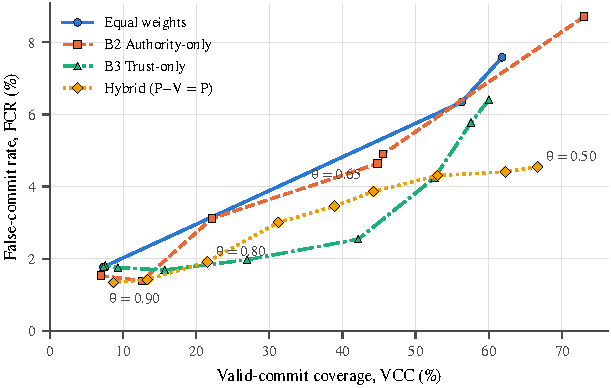
\includegraphics[]{fig2_threshold_tradeoff.pdf}\caption{Commit-threshold trade-off after Revenue degrades (S2): false-commit rate against valid-commit coverage as $\theta$ varies from 0.50 to 0.90 in steps of 0.05 (means over 100 seeds, ideal feedback)}\end{figure}
\subsection*{5.3 RQ3: Availability and coverage}
With 25\% outages, the hybrid's FCR was 1.13\%, but it committed only 31.8\% of valid requests, against majority's 44.6\% (H3; precision target missed). In the pre-specified q\_min sweep, lowering q\_min to 0 raised the hybrid's VCC to 60.5\% and its FCR to 2.70\%. Section 5.6 shows that most of this coverage gap comes from the gate.

\subsection*{5.4 RQ4: The proceedings veto}
P and P--V made identical decisions in every seed of S5a and S5b (H4), as Sect. 3.6 predicts. The Judiciary's learned trust on restr stayed between 0.67 and 1.0, outside the window where the veto could act. This holds for the tested authority matrices, threshold and trust trajectories only.

The stress test still separated the other mechanisms. In S5a, breaches per 1,000 requests were 50.6 for majority, 32.8 for trust-only, 2.3 for authority-only and 2.2 for the hybrid. Table 4 shows one such case.

\subsection*{5.5 RQ5: Realistic feedback}
H5, that realistic feedback would raise FCR, was not supported (Holm p = 1.00). The two-sided interval lies just below zero. An exploratory two-sided test gives p = 0.042 unadjusted; this would not survive adjustment within the family of seven, so we report no reliable difference in either direction.

Under F1, trust learns mostly from escalated, contested requests. In a 10-seed diagnostic, this selection bias lowered the Sub-Registrar's trust on own from about 0.80 to 0.60. The effect fades as the label delay grows (Fig. 3).

\begin{figure}[tb]\centering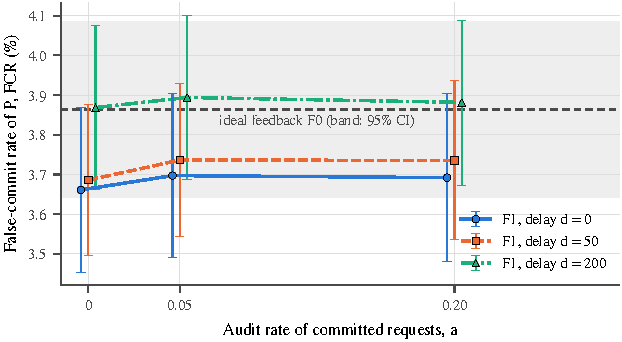
\includegraphics[]{fig3_feedback.pdf}\caption{False-commit rate of P under realistic feedback F1 in S2, by audit rate and label delay; whiskers are between-seed 95\% CIs, the dashed line and band show ideal feedback F0}\end{figure}
\subsection*{5.6 Exploratory: coverage-gate ablation (A1)}
This analysis was specified in addendum A1, committed before it ran but after the main results were seen. Every mechanism was re-run on seeds 1–100 under three gates:

\begin{itemize}
\item G0: no gate.
\item G1: a common gate of at least 2 of 3 offices responding.
\item G2: the main-study gates, which reproduced the main results exactly.
\end{itemize}
% Auto-generated by paper_assets/build_assets.py from saved results -- do not edit numbers by hand.
% Preamble needs: \usepackage{booktabs,array,tabularx,makecell}
\begin{table}[tb]
\centering
\caption{Exploratory coverage-gate ablation A1 (paired 95\% CIs, 100 seeds, percentage points)}\label{tab:ablation}
\footnotesize
\setlength{\tabcolsep}{3pt}
\renewcommand{\arraystretch}{1.1}
\begin{tabularx}{\textwidth}{@{}>{\raggedright\arraybackslash}Xccc@{}}
\toprule
Comparison & Scenario & FCR difference & VCC difference \\
\midrule
Hybrid $-$ majority, no gate (G0) & S1 & $-$1.85 [$-$2.00, $-$1.69] & $-$0.27 [$-$0.53, $-$0.004] \\
Hybrid $-$ majority, no gate (G0) & S4 & $-$0.99 [$-$1.14, $-$0.83] & +8.41 [+8.13, +8.70] \\
Hybrid $-$ majority, common count gate (G1) & S1 & $-$1.85 [$-$2.01, $-$1.70] & $-$0.27 [$-$0.53, $-$0.004] \\
Hybrid $-$ majority, common count gate (G1) & S4 & $-$1.01 [$-$1.19, $-$0.83] & +8.41 [+8.13, +8.70] \\
Hybrid: weighted gate $-$ count gate & S1 & $-$0.11 [$-$0.15, $-$0.07] & $-$4.25 [$-$4.39, $-$4.11] \\
Hybrid: weighted gate $-$ count gate & S4 & $-$0.72 [$-$0.85, $-$0.60] & $-$21.23 [$-$21.52, $-$20.95] \\
\bottomrule
\end{tabularx}
\end{table}

Under a common gate, the hybrid's FCR advantage over majority is about as large as in the main study. Its coverage is almost the same as majority's in S1 and 8.4 points higher in S4.

The main-study coverage gap therefore comes mainly from the weighted gate. That gate is stricter than two of three, because it effectively requires the Judiciary for restr. In return, it removes a further 0.11 to 0.72 points of FCR. No weighted mechanism ever committed a request in which a check had a single responder.

\subsection*{5.7 Exploratory: robustness study (A2)}
Addendum A2 was committed before it ran. It stated in advance that all its results would be reported. It varies one assumption at a time on seeds 1–100 and asks whether three conclusions survive:

\begin{itemize}
\item C1: the hybrid is below majority.
\item C2: the hybrid is below authority-only after degradation.
\item C3: trust-only is below the hybrid in S2.
\end{itemize}
Of 68 checks, 67 held, one weakened and none reversed (Table 10).

% Auto-generated by paper_assets/build_assets.py from saved results -- do not edit numbers by hand.
% Preamble needs: \usepackage{booktabs,array,tabularx,makecell}
\begin{table}[tb]
\centering
\caption{Exploratory robustness study A2: levels at which each main conclusion holds, with the range of FCR differences in points}\label{tab:robustness}
\footnotesize
\setlength{\tabcolsep}{3pt}
\renewcommand{\arraystretch}{1.1}
\begin{tabularx}{\textwidth}{@{}>{\raggedright\arraybackslash}Xcccc@{}}
\toprule
Factor varied & C1 (S1) & C1 (S2) & C2 & C3 \\
\midrule
Off-home accuracy 0.60--0.85 & \makecell{4/4 \\ ($-$6.2 to $-$0.4)} & \makecell{4/4 \\ ($-$4.9 to $-$1.4)} & \makecell{3/4 \\ ($-$1.6 to $-$0.2)} & \makecell{4/4 \\ ($-$1.3 to $-$0.8)} \\
Home accuracy 0.85--0.95 & \makecell{3/3 \\ ($-$2.0 to $-$0.9)} & \makecell{3/3 \\ ($-$2.5 to $-$1.6)} & \makecell{3/3 \\ ($-$1.3 to $-$1.1)} & \makecell{3/3 \\ ($-$1.9 to $-$1.3)} \\
Shared R+S errors $\rho$ = 0--0.20 & \makecell{4/4 \\ ($-$3.6 to $-$2.0)} & \makecell{4/4 \\ ($-$3.6 to $-$2.5)} & \makecell{4/4 \\ ($-$2.0 to $-$1.3)} & \makecell{4/4 \\ ($-$5.0 to $-$1.3)} \\
Label noise e = 0--0.10, F0 & --- & \makecell{4/4 \\ ($-$2.5 to $-$2.4)} & \makecell{4/4 \\ ($-$1.3 to $-$1.1)} & \makecell{4/4 \\ ($-$1.3 to $-$1.2)} \\
Label noise e = 0--0.10, F1 & --- & \makecell{4/4 \\ ($-$2.6 to $-$2.5)} & \makecell{4/4 \\ ($-$1.6 to $-$1.4)} & \makecell{4/4 \\ ($-$0.9 to $-$0.8)} \\
\bottomrule
\end{tabularx}
\par\smallskip
\parbox{\textwidth}{\scriptsize C1: hybrid below majority. C2: hybrid below authority-only after degradation (requests 251--1000). C3: trust-only below hybrid (S2). Holds: the 95\% CI excludes 0 with the main-study sign. No conclusion reversed.}
\end{table}

The weakened check is C2 at off-home accuracy 0.60, where the difference was --0.15 points [--0.39, +0.09]. When offices are that unreliable outside their own check, the hybrid and authority-only are not distinguishable after degradation.

Shared errors kept the ranking but raised every rate (Fig. 4b). At $\rho$ = 0.20, the hybrid's FCR in S1 rose from 1.09\% to 8.33\%, against 11.93\% for majority. Label noise up to 10\% barely moved the hybrid under realistic feedback, from 3.74\% to 3.80\% (Fig. 4c).

\begin{figure}[tb]\centering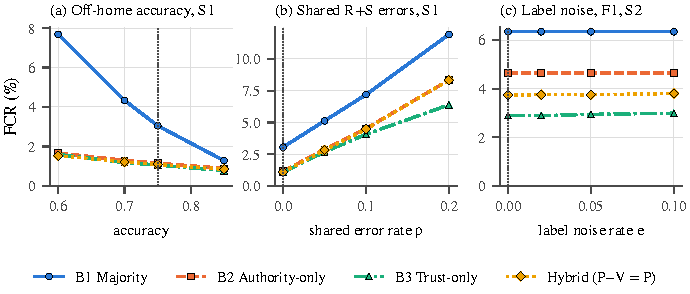
\includegraphics[]{fig4_robustness.pdf}\caption{Exploratory robustness study A2 (100 seeds): false-commit rate by mechanism as (a) off-home accuracy, (b) the shared error rate of Revenue and Sub-Registrar and (c) label noise vary; dotted lines mark the main-study settings}\end{figure}
\section*{6 Discussion}
Under the stated assumptions, the results support weighting conflicting evidence rather than counting votes. They do not support calling the hybrid the best rule.

What the results show.

\begin{itemize}
\item Authority-aware weighting accounts for most of the gain over majority voting. The gain does not depend on the coverage gate (Table 9), and it held at every level of the robustness study (Table 10).
\item Learned trust adds protection when authority is wrong or degrades. This holds under ideal feedback; realistic feedback distorts trust through selection bias.
\item The veto did not change any decision under the tested configurations. This does not show that a separate override for legal proceedings is unnecessary. The model abstracts what a reported proceeding means, whether it is authentic and whether it binds the requested change.
\end{itemize}
The hybrid's position. Authority and trust are multiplied, so an office with high authority keeps substantial weight after its trust falls toward chance. That is why trust-only was safer after Revenue degraded. Trust-only, with no prior on which office should know what, escalates more in normal operation. An above-chance trust transform, T' = max(0, 2T -- 1), would remove the weight of an office reporting at chance. It was outside the frozen protocol and is left to future work.

Coverage is a policy choice. The weighted gate buys a small further reduction in false commits at a large cost in coverage, especially under outages (--21 points of VCC in S4). A simple two-of-three gate kept nearly all of the weighting's safety gain. Which gate to use depends on the cost of a wrong ledger entry against the cost of a manual review, which we could not source.

Shared errors are the main weakness. Weighting cannot detect two offices that are confidently wrong together. In the robustness study, one stale record copied by Revenue and Sub-Registrar in 20\% of checks raised the hybrid's FCR almost eightfold in S1. The ranking survived, but the absolute safety did not. Any real use would need independent evidence for at least one check, or explicit detection of copied records.

Review load. Every weighted mechanism escalated about half of all requests in S1, while 28.8\% were invalid. The causes are low off-domain accuracy and the need to pass three checks.

Threats to validity.

\begin{itemize}
\item Synthetic data. All accuracies, failure rates and outage rates are assumed, and Table 2's signals are illustrative. A2 shows the relative conclusions survive a range of values, not that the values are realistic.
\item Legal scope. The model is inspired by selected mutation conditions [12]. It omits record stability and does not decide title [16].
\item Dependence. Outages are independent, and errors are independent except in A2's shared-error test.
\item Feedback. Main results assume immediate, error-free labels; A2 relaxes only label accuracy.
\item Design alignment. S1 aligns authority with accuracy by design; S3 tests one misalignment.
\item Precision and analysis. H2b and H3 missed the precision target. Five analysis choices fell outside the protocol (Table 12). A1, A2 and the two-sided H5 test are exploratory.
\end{itemize}
\section*{7 Conclusion}
We studied a synthetic pre-commit validation policy for requested ownership changes. It bundles three simulated checks, weights each office's report by claim-specific authority and learned trust, and escalates rather than rejects.

In 100 paired runs per scenario, it cut false commits about threefold against majority voting, a gain that persisted under a common coverage gate and across every robustness level tested. It made fewer false commits than authority-only weighting when the most authoritative office degraded or was misassigned. Trust-only weighting was safer still, at a cost in coverage. The proceedings veto never changed a decision in the configurations tested. Shared errors between offices were the clearest weakness: the ranking held, but every method's false-commit rate rose sharply.

None of this describes real land offices, and none of it bears on title.

Future work:

\begin{itemize}
\item detecting copied or correlated records;
\item an above-chance trust transform;
\item grounding parameters in verified Gujarat sources;
\item response delays;
\item adversarial sources and forged documents;
\item chaincode integration.
\end{itemize}
\section*{Appendix A: Result status and analysis choices}
% Auto-generated by paper_assets/build_assets.py from saved results -- do not edit numbers by hand.
% Preamble needs: \usepackage{booktabs,array,tabularx,makecell}
\begin{table}[tb]
\centering
\caption{Status of every result}\label{tab:status}
\footnotesize
\setlength{\tabcolsep}{3pt}
\renewcommand{\arraystretch}{1.1}
\begin{tabularx}{\textwidth}{@{}>{\raggedright\arraybackslash}p{4.8cm}>{\raggedright\arraybackslash}X@{}}
\toprule
Result & Status \\
\midrule
Tables 7--8; Figs. 2--3; $q_{\min}$ sweep & Pre-specified (frozen protocol); five analysis choices in Table 12 \\
Veto bound (Sect. 3) & Analytic, derived before the protocol freeze \\
Counts per 1,000 requests; quoted trust values & Descriptive re-expression of pre-specified runs \\
Two-sided test for H5 & Exploratory, added after results were seen \\
Table 9 (A1); Table 10 and Fig. 4 (A2) & Exploratory; addenda committed before running \\
\bottomrule
\end{tabularx}
\end{table}

% Auto-generated by paper_assets/build_assets.py from saved results -- do not edit numbers by hand.
% Preamble needs: \usepackage{booktabs,array,tabularx,makecell}
\begin{table}[tb]
\centering
\caption{Analysis choices not covered by the frozen protocol (accepted by the supervisor)}\label{tab:notes}
\footnotesize
\setlength{\tabcolsep}{3pt}
\renewcommand{\arraystretch}{1.1}
\begin{tabularx}{\textwidth}{@{}c>{\raggedright\arraybackslash}p{4.2cm}>{\raggedright\arraybackslash}X@{}}
\toprule
\# & Situation & Choice \\
\midrule
1 & H4 has zero variance & Interval is the point 0; p = 1.0 in the Holm family \\
2 & H1b has no direction & Two-sided test inside the Holm family of seven \\
3 & Significant and inside $\pm$$\Delta$ (H1b) & Worded `lower, but smaller than $\Delta$' \\
4 & CI opposite a one-sided hypothesis (H5) & `Not supported'; two-sided CI and exploratory test reported \\
5 & H3 has no direction & Worded from its unadjusted CI; labelled descriptive \\
\bottomrule
\end{tabularx}
\end{table}

These choices were made during analysis, after the 30-seed results were first computed, and were accepted by the supervisor on 28 Oct 2026.

\section*{References}\footnotesize
\begin{enumerate}
\item V. Thakur, M. N. Doja, Y. K. Dwivedi, T. Ahmad, and G. Khadanga, "Land records on Blockchain for implementation of Land Titling in India," Int. J. Inf. Manage., vol. 52, Art. no. 101940, Jun. 2020, doi: 10.1016/j.ijinfomgt.2019.04.013.
\item E. Androulaki et al., "Hyperledger Fabric: A distributed operating system for permissioned blockchains," in Proc. 13th EuroSys Conf., Porto, Portugal, Apr. 2018, doi: 10.1145/3190508.3190538.
\item G. Caldarelli, "Understanding the blockchain oracle problem: A call for action," Information, vol. 11, no. 11, Art. no. 509, Oct. 2020, doi: 10.3390/info11110509.
\item H. Al-Breiki, M. H. U. Rehman, K. Salah, and D. Svetinovic, "Trustworthy blockchain oracles: Review, comparison, and open research challenges," IEEE Access, vol. 8, pp. 85675–85685, 2020, doi: 10.1109/ACCESS.2020.2992698.
\item S. Soner, R. Litoriya, and P. Pandey, "Exploring blockchain and smart contract technology for reliable and secure land registration and record management," Wireless Pers. Commun., vol. 121, no. 4, pp. 2495–2509, Dec. 2021, doi: 10.1007/s11277-021-08833-1.
\item M. Shuaib, S. M. Daud, S. Alam, and W. Z. Khan, "Blockchain-based framework for secure and reliable land registry system," TELKOMNIKA, vol. 18, no. 5, pp. 2560–2571, Oct. 2020, doi: 10.12928/TELKOMNIKA.v18i5.15787.
\item A. Sahai and R. Pandey, "Smart contract definition for land registry in blockchain," in Proc. IEEE 9th Int. Conf. Commun. Syst. Netw. Technol. (CSNT), Gwalior, India, 2020, pp. 230–235, doi: 10.1109/CSNT48778.2020.9115752.
\item A. Hassan, I. Makhdoom, W. Iqbal, A. Ahmad, and A. Raza, "From trust to truth: Advancements in mitigating the blockchain oracle problem," J. Netw. Comput. Appl., vol. 217, Art. no. 103672, Aug. 2023, doi: 10.1016/j.jnca.2023.103672.
\item S. K. Lo, X. Xu, M. Staples, and L. Yao, "Reliability analysis for blockchain oracles," Comput. Electr. Eng., vol. 83, Art. no. 106582, 2020. [VERIFY DOI]
\item L. Breidenbach et al., "Chainlink 2.0: Next steps in the evolution of decentralized oracle networks," Chainlink Labs, white paper v1.0, Apr. 15, 2021. [Online]. Available: https://research.chain.link/whitepaper-v2.pdf
\item A. Josang, R. Ismail, and C. Boyd, "A survey of trust and reputation systems for online service provision," Decis. Support Syst., vol. 43, no. 2, pp. 618–644, Mar. 2007, doi: 10.1016/j.dss.2005.05.019.
\item Government of Gujarat, Revenue Dept., "The Gujarat Land Revenue (Amendment) Ordinance, 2026," Gujarat Ordinance No. 1 of 2026, Gujarat Government Gazette, Extraordinary, Part IV, Extra No. 6, Mar. 31, 2026. [VERIFY: whether replaced by an Act]
\item Y. Li et al., "A survey on truth discovery," arXiv:1505.02463, 2015. [VERIFY: journal version]
\item Y. Xiao, N. Zhang, W. Lou, and Y. T. Hou, "A decentralized truth discovery approach to the blockchain oracle problem," in Proc. IEEE INFOCOM, 2023, pp. 1–10. [VERIFY DOI]
\item A. Khanna, P. Singh, and P. K. Angra, "Blockchain-enabled e-governance framework for secure and transparent land record management," Int. Res. J. Multidiscip. Technovation, vol. 8, no. 4, pp. 73–90, 2026, doi: 10.54392/irjmt2645.
\item Jitendra Singh v. State of M.P., 2021 SCC OnLine SC 802 (Sept. 6, 2021); see also Tarachandra v. Bhawarlal, 2025 INSC 1485. [VERIFY: judgment texts]
\end{enumerate}
LNCS uses its own reference style (numbered, Springer format). Convert these IEEE-style entries with the template's bibliography style; keep the DOIs.

\end{document}
